\documentclass[conference,onecolumn]{IEEEtran}
\usepackage{enumitem}
\usepackage{cite}
\usepackage{graphicx}
\usepackage{float}
\usepackage{amsmath, nccmath, bm}
\usepackage{amssymb}
\graphicspath{{./images}}

\title{XM Radio Reception with the PlutoSDR}

\author{
\IEEEauthorblockN{Owen Sowatzke}
\IEEEauthorblockA{\textit{Electrical Engineering Department} \\
\textit{University of Arizona}\\
Tucson, USA \\
osowatzke@arizona.edu}
\and
\IEEEauthorblockN{Glenn Alan Walker}
\IEEEauthorblockA{\textit{Electrical Engineering Department} \\
\textit{University of Arizona}\\
Tucson, USA \\
gaw@arizona.edu}}

\begin{document}
\maketitle

% Proposal
% XM radio leverages a combination of satellites and terrestrial repeaters to diversify its transmitted signal. The satellites transmit QSPK-modulated symbols, and the terrestrial repeaters leverage COFDM modulation \cite{5586866}. For our final project, we propose demodulating the signal from a single satellite and performing forward error correction (FEC). Our project will leverage the time, frequency, and frame synchronization methods covered in class. Additionally, it will extend the material covered in class to forward error correction. XM radio is a proprietary signal, and the technical details are documented only in patents such as \cite{a2008_us8260192b2, marko_2012_us8667344b2}. Major milestones for our project include: performing timing and frequency synchronization, extracting the master frame preamble (MFP) and frame synchronization preamble (FSP), and demodulating the signal from a single satellite. Additional stretch goals that will be addressed only if time permits include: demodulating the COFDM signals from terrestrial repeaters, combining the returns from multiple satellites and/or the terrestrial repeaters, and playing XM channel 1 audio (free preview channel). We believe that this project will reinforce what we learned in the course and provide invaluable experience performing FEC and OFDM demodulation.

\begin{abstract}
	In this project, we perform XM radio demodulation and forward error correction (FEC) in GNU radio using data captured with the Pluto SDR. GNU radio allows us to easily experiment with XM radio and rapidly prototype new receiver architectures. In our work, we concentrate on the time-domain multiplexed (TDM) satellite signals. To demodulate the signal, we leverage concepts learned in the class such as timing synchronization, carrier synchronization, and frame synchronization. As part of FEC, we also perform time deinterleaving, Virterbi decoding, and Reed Solomon Decoding.
\end{abstract}

\section{Introduction}

In this project, we demodulate XM radio transmissions and perform forward error correction (FEC) with our Pluto SDR. XM radio uses a combination of satellites and terrestrial repeaters to diversify its transmitted signal. The satellites use QPSK modulation, and the terrestrial repeaters use coded orthogonal frequency domain multiplexing (COFDM). Our work focuses on the time-division multiplexed (TDM) signal from a single satellite. To demodulate this signal we leverage concepts from the course such as time synchronization, carrier synchronization, and frame synchronization. We also perform FEC, which was not covered in the course. With respect to FEC, we perform time deinterleaving, Virterbi decoding, and Reed Solomon Decoding. Because XM radio is a proprietary signal, it is documented only in patents such as \cite{a2008_us8260192b2, marko_2012_us8667344b2}. However, the patents leave out portions of the details, which require us to reverse-engineer portions of the system.

\section{Background}

In this section, we provide background information on XM radio modulation. XM radio divides their content across two separate ensembles (Ensemble A and Ensemble B), which are illustrated in Figure \ref{fig::xm_satellite_config}. Each ensemble contains half of the XM radio channels and uses transmitter diversity to improve signal quality and prevent dropouts. The diversity scheme specifically uses QPSK-modulated signals from two separate satellites and a terrestrial COFDM-modulated signal.

\iffalse
\begin{figure}[H]
	\centerline{\fbox{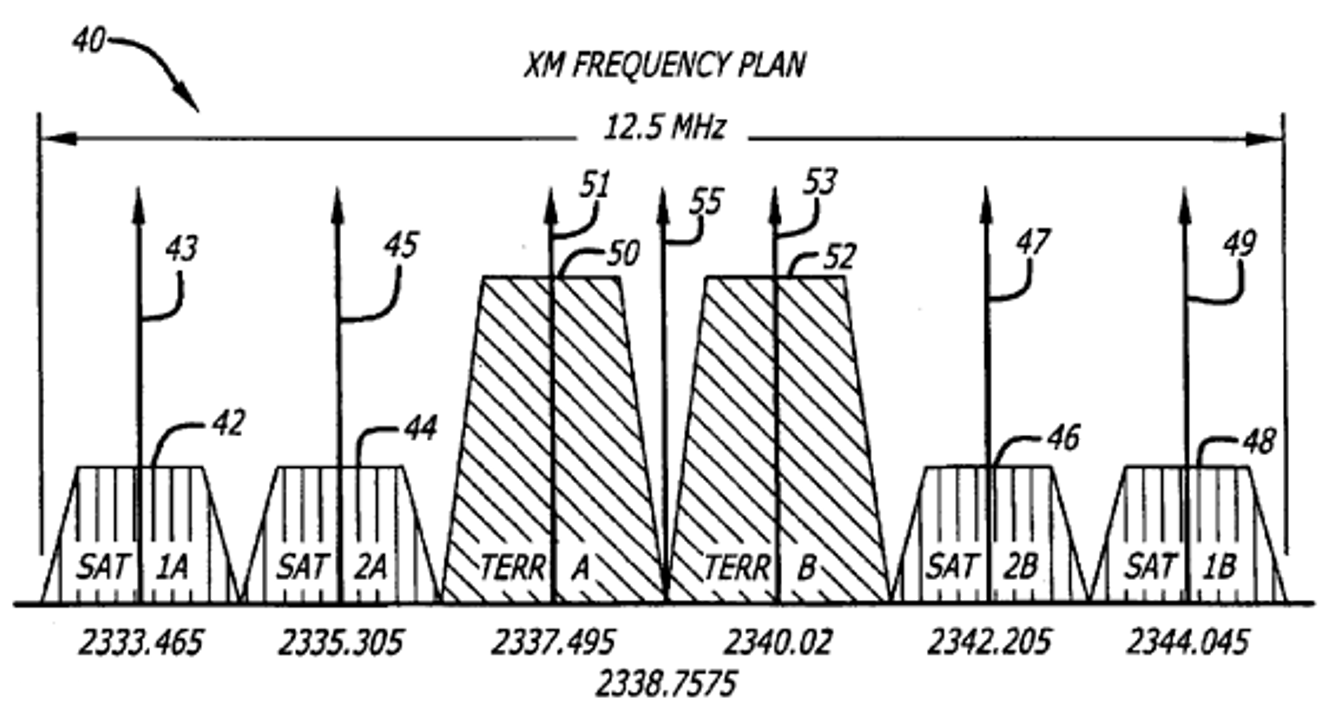
\includegraphics[width=0.5\textwidth]{xm_spectrum.png}}}
	\caption{XM Radio Spectrum \cite{a1999_us6724827b1}}
	\label{fig::xm_spectrum}
\end{figure}
\fi

\begin{figure}[H]
	\centerline{\fbox{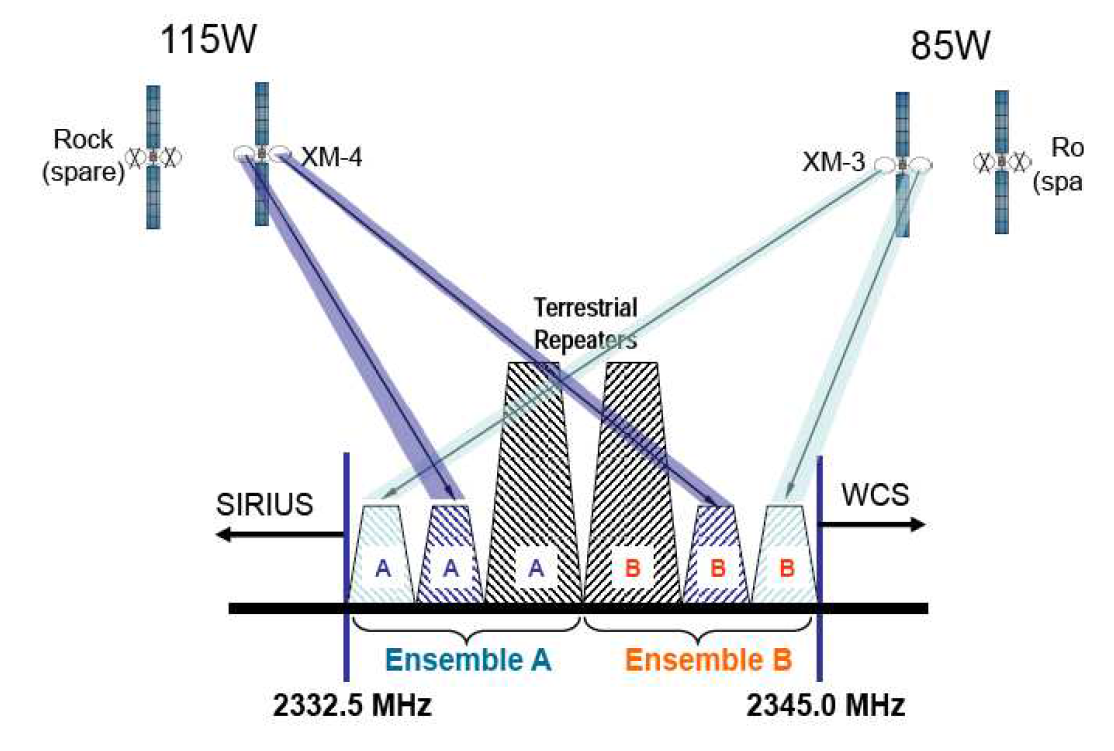
\includegraphics[width=0.5\textwidth]{xm_satellite_config.png}}}
	\caption{XM Radio Satellite Configuration \cite{5586866}}
	\label{fig::xm_satellite_config}
\end{figure}

\noindent The center frequencies and bandwidths for each subregion of the spectrum are given in Table \ref{table::center_freq_and_bw}:
\vspace{-12pt}
\begin{table}[H]
	\begin{center}
	\caption{XM Radio Center Frequencies and Bandwidths \cite{andreas_2010_us8594559b2}}
	\label{table::center_freq_and_bw}
	\begin{tabular}{| c | c | c |}
		\hline
		\textbf{Name} & $\mathbf{f_c}$ & \textbf{BW}\\
		\hline
		SAT1A	& 2333.465 MHz & 1.886 MHz\\
		\hline
		SAT2A	& 2335.305 MHz & 1.886 MHz\\
		\hline
		TERRA & 2337.490 MHz & 2.51 MHz \\
		\hline
		TERRB & 2340.020 MHz & 2.51 MHz \\
		\hline
		SAT1B	& 2342.205 MHz & 1.886 MHz\\
		\hline
		SAT2B	& 2344.045 MHz & 1.886 MHz\\
		\hline
	\end{tabular}
	\end{center}
\end{table}

% We concentrate specifically on the TDM receiver. An example of its architecture is displayed in Figure
% \ref{fig::tdm_receiver}.

% XM Radio divides their content across two separate ensembles (Ensemble A and Ensemble B), which are illustrated in Figure \ref{fig::xm_satellite_config}. Each ensemble uses transmitter diversity to improve signal quality and prevent dropouts. The diversity scheme specifically uses QPSK-modulated signals from two separate satellites and a terrestrial COFDM-modulated signal. We concentrate specifically on the TDM receiver. An example of its architecture is displayed in Figure \ref{fig::tdm_receiver}. 

\iffalse
\begin{figure}[H]
	\centerline{\fbox{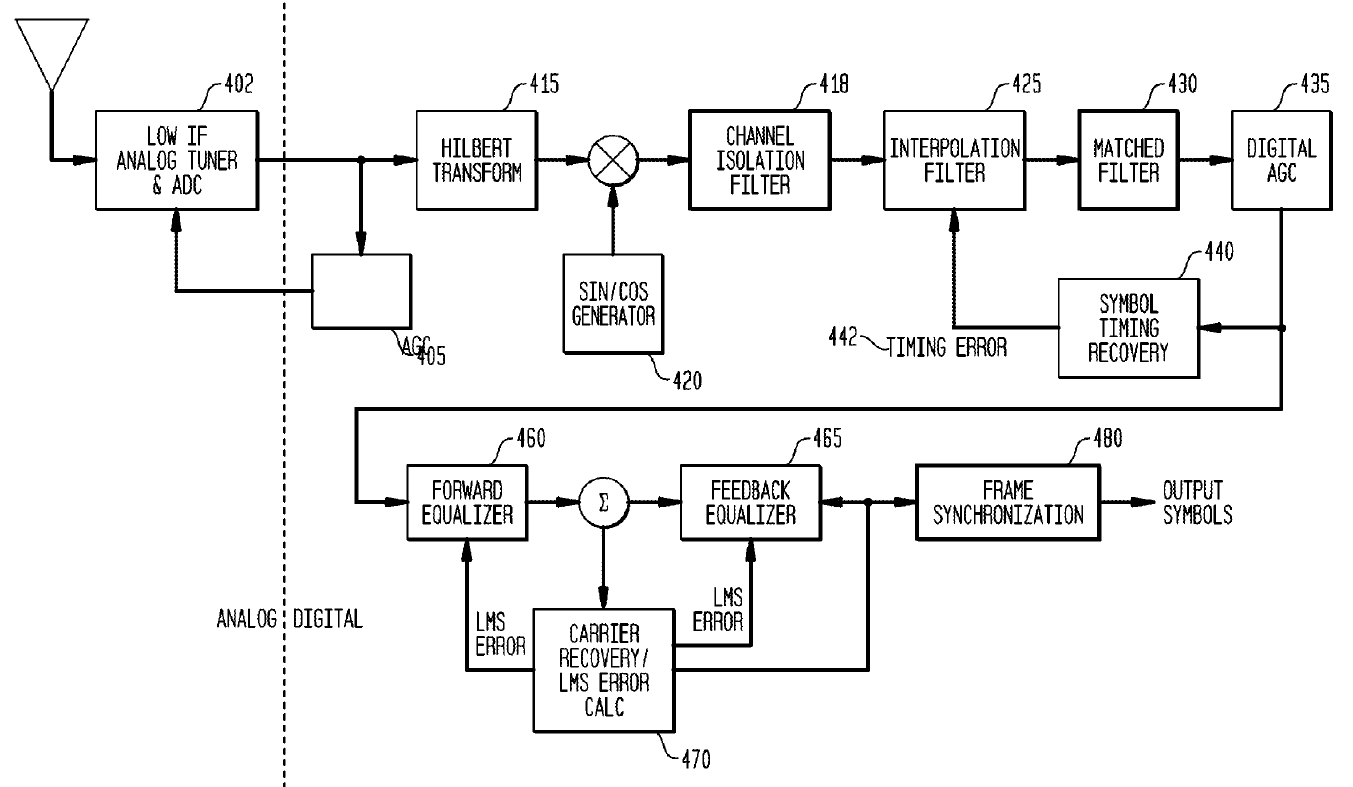
\includegraphics[width=0.5\textwidth]{tdm_receiver.png}}}
	\caption{TDM Receiver Architecture \cite{a2008_us8260192b2}}
	\label{fig::tdm_receiver}
\end{figure}
\fi

In this report, we concentrate specifically on the SAT channels (TDM channels). A sample TDM receiver architecture is shown in Figure \ref{fig::tdm_receiver_architecture}. In this architecture, We start by performing coarse frequency compensation to remove large carrier offsets. Next, we pass the signal through a matched filter to maximize the SNR. Then, we perform timing recovery to ensure we are sampling the symbols in the ideal positions (midway between symbol transitions). We also perform carrier recovery to get rid of any residual phase or frequency offsets. Finally, we perform frame synchronization to form frames of data with the correct set of samples.

\begin{figure}[H]
	\centerline{\fbox{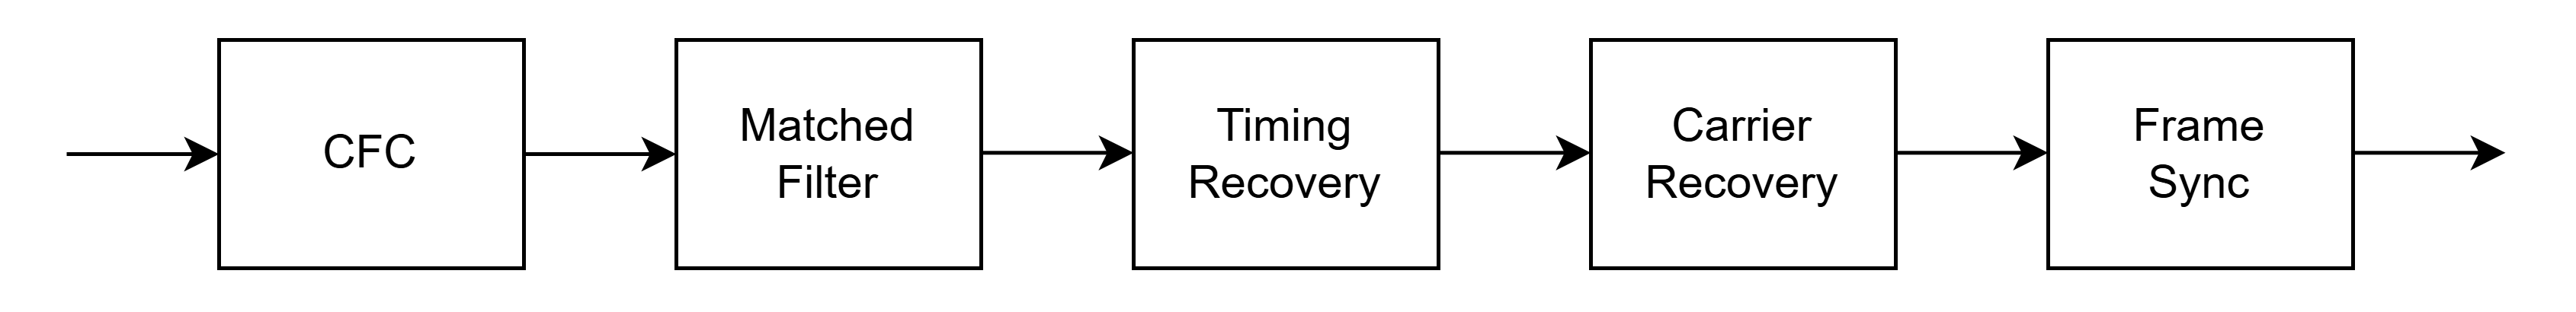
\includegraphics[width=0.8\textwidth]{tdm_receiver_architecture.png}}}
	\caption{TDM Receiver Architecture}
	\label{fig::tdm_receiver_architecture}
\end{figure}

\subsection{Coarse Frequency Compensation}

We can write our base band signal with a frequency offset $f_o$ as follows:

\begin{equation}
	r(k) = s(k)e^{j(2{\pi}f_okT + \theta)}
\end{equation}

\noindent Additionally, for PSK modulated signals we know that the amplitude $s(k)$ is constant and the phase $\theta$ is defined as:

\begin{equation}
	\theta = \frac{2{\pi}n}{M},\quad n \in 0,1,...,M-1
\end{equation}

\noindent where $M$ is the constellation order. If we raise our received data to the M-th power, we can strip the modulation from our received data.

\begin{equation}
	r^M(k) = s^M(k)e^{j(2{\pi}f_okT + \theta)M} = s^M(k)e^{j2{\pi}Mf_okT}
\end{equation}

\noindent As previously stated, we can ignore the constant $s^M(k)$ term for PSK modulation. Then if we take an FFT of our data, we should be left with a sinc function centered about $Mf_oT$. In other words, we can solve for the coarse frequency offset as follows:

\begin{equation}
	\hat{f}_o = \frac{1}{MTK}\text{arg}\left|\sum_{k=0}^{K-1}{r^M(k)e^{-j2{\pi}kT/K}}\right|
\end{equation}

\noindent Then, we can feed a negated copy of the coarse frequency offset ($-\hat{f}_o$) into an NCO and remove the coarse frequency offset. Following the work of \cite{collins_2018_softwaredefined}, the coarse frequency offset correction is placed at the start of the chain to ensure that it operates on the largest possible bandwidth.
 
\subsection{Timing Synchronization}

Nyquist filters are used to minimize intersymbol interference (ISI). The impulse response of a Nyquist filter is zero at symbol intervals (i.e. $h(nT_s) = 0 \ \forall\ n \neq 0$). A sinc function is a type I Nyquist filter and has a perfectly bandlimited frequency response. However, the impulse response is infinite time and decays with $1/t$, which does not converge in the presence of intersymbol errors. As a result, we typically use a type II Nyquist filter, which has a finite impulse response that decays faster with time. However, type II Nyquist filters are not perfectly bandlimited in the frequency domain and have some rolloff and excess bandwidth. A common Nyquist filter is the square-root raised cosine (SRRC) filter, which is defined as follows:
 
\begin{equation}
	h(t) = \begin{cases}
		\dfrac{1}{\sqrt{T_s}}\left(1 - \beta + 4\dfrac{\beta}{\pi}\right), & t = 0 \\[12pt]
		\dfrac{\beta}{\sqrt{2T_s}}\left[\left(1 + \dfrac{2}{\pi}\right)\sin\left(\dfrac{\pi}{4\beta}\right)+ \left(1-\dfrac{2}{\pi}\right)\cos\left(\dfrac{\pi}{4\beta}\right)\right], & t = \pm\dfrac{T_s}{4\beta} \\[12pt]
		\dfrac{1}{\sqrt{T_s}}\dfrac{\sin\left[\pi\dfrac{t}{T_s}(1-\beta)\right]+4\beta\dfrac{t}{T_s}\cos\left[\pi\dfrac{t}{T_s}(1+\beta)\right]}{\pi\dfrac{t}{T_s}\left[1 - \left(4\beta\dfrac{t}{T_s}\right)^2\right]}, & \text{otherwise}
	\end{cases}
	\label{eq::srrc_filter}
\end{equation}

\noindent Nyquist filters only result in zero ISI, when they are properly sampled at the midpoint of symbol transitions. Timing synchronization is used to compensate for imperfect sampling. The timing synchronization algorithm is illustrated in Figure \ref{fig::timing_synchronization}.

\begin{figure}[H]
	\centerline{\fbox{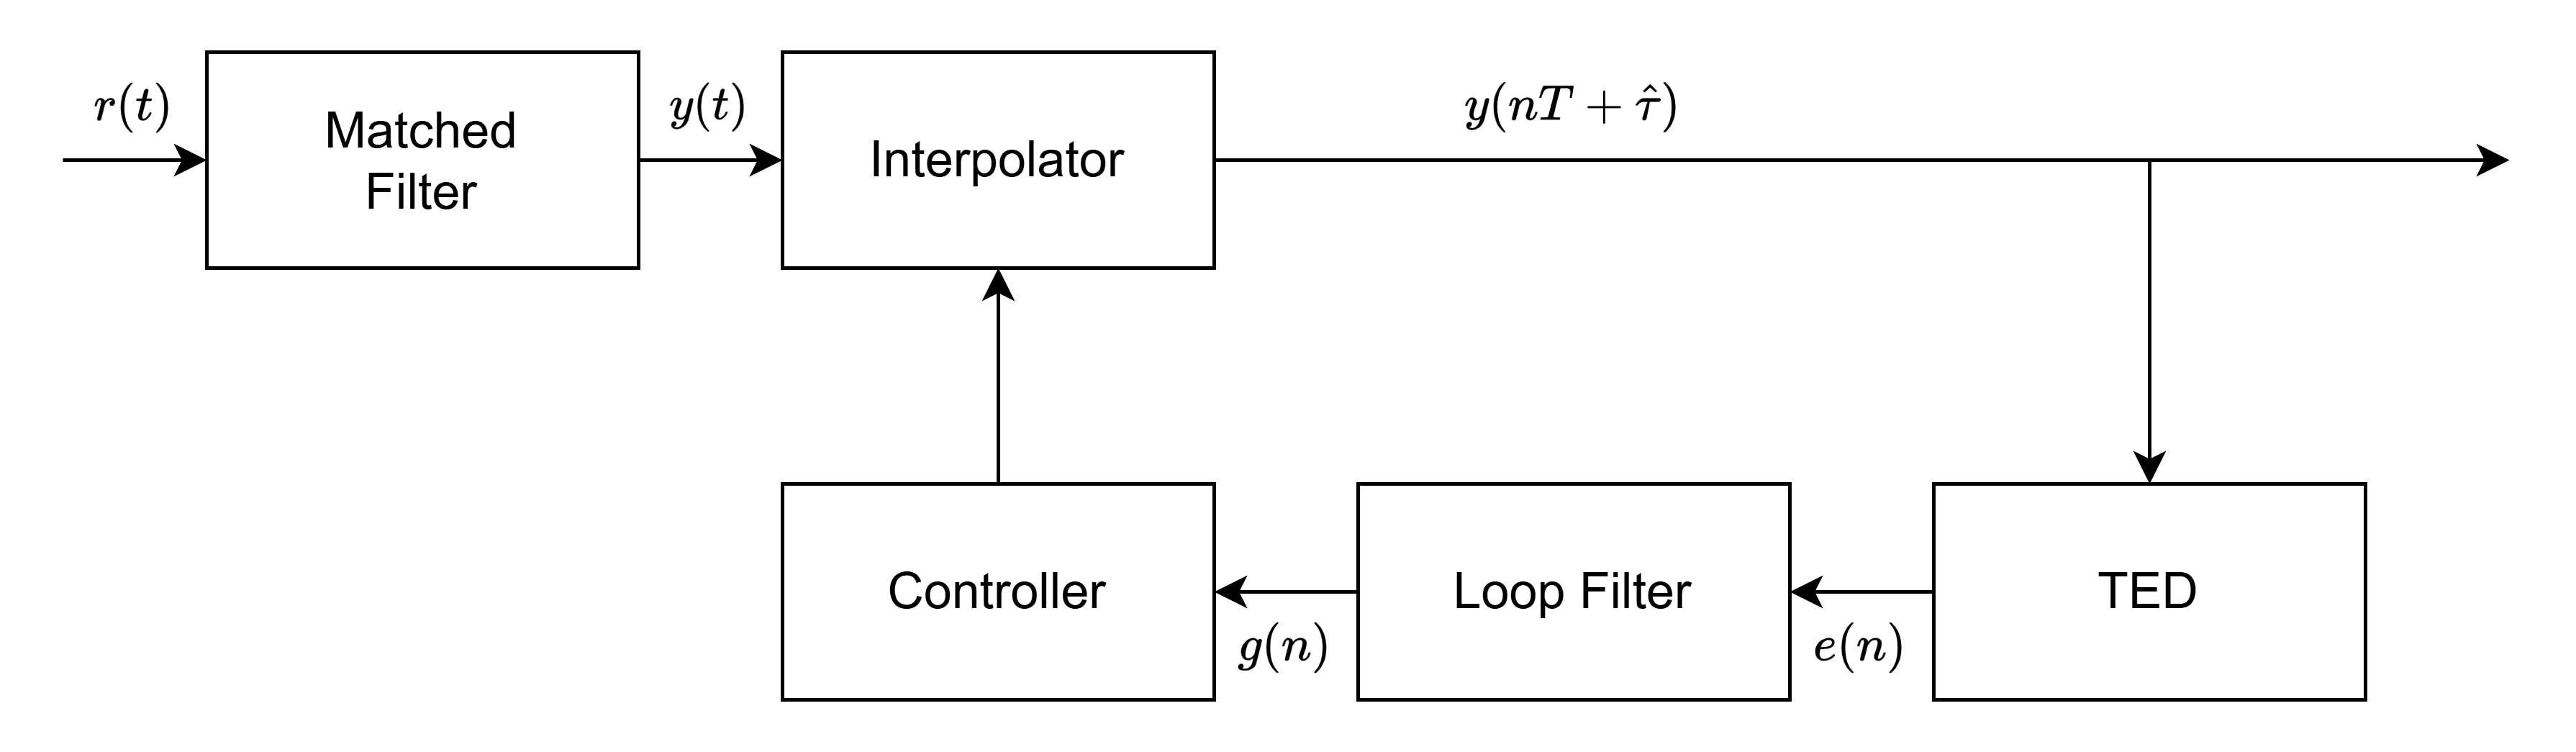
\includegraphics[width=0.6\textwidth]{timing_synchronization.png}}}
	\caption{Timing Synchronization Block Diagram}
	\label{fig::timing_synchronization}
\end{figure}

\subsubsection{Interpolator}

\noindent The interpolator applies a fractional delay to the input samples. We specifically use a piecewise polynomial filter (PPF), which interpolates the input data as follows:

\begin{equation}
	x(kT_s + \mu(k)T_s) = \sum_{n=-2}^{1}{h(n)x((k-n)T_s)}
\end{equation}

\noindent where the filter taps $h(n)$ are given by

\begin{equation}
\begin{split}
	h = [&\alpha\mu(k)(\mu(k) - 1), \\
	&-\alpha\mu(k)^2 - (1-\alpha)\mu(k) + 1,\\
	&-\alpha\mu(k)^2 + (1+\alpha)\mu(k),\\
	&\alpha\mu(k)(\mu(k) - 1)]
\end{split}
\end{equation}

\subsubsection{Timing Error Detector}

\noindent The timing error detector (TED) measures the timing offset in the data. There are a few different methods for measuring these offsets. They include the zero crossing, Gardener, and  M\"{u}ller and Mueller methods. In the work that follows, we use the Gardener method because it is least sensitive to carrier phase offsets. The gardener method defines the error signal $e(k)$ as follows:

\begin{equation}
\begin{split}
	e(k) =& \text{Re}(x((k-1/2)T_s+\tau))\left[\text{Re}(x((k-1)T_s + \tau)) - \text{Re}(x(kT_s + \tau))\right] + \\
	&\text{Im}(x((k-1/2)T_s+\tau))\left[\text{Im}(x((k-1)T_s+\tau)) -\text{Im}(x(kT_s+\tau))\right]
\end{split}
\end{equation}

\subsubsection{Loop Filter}

\noindent The timing error detector output is then fed into a loop filter which produces a stable signal for the controller. The loop filter uses a proportional integral (PI) filter, which is defined as follows:

\begin{equation}
	y(n) = G_1x(n) + G_2\sum_{k=0}^{n}{x(k)}
\end{equation}

\noindent In the above equations, $G_1$ and $G_2$ are constants and can be expressed in terms of the normalized loop bandwidth ($B_{\text{Loop}}$), the damping factor ($\zeta$), the samples per symbol ($N$), and the detector gain ($G_D$). They are specifically defined as follows:

\begin{align}
	G_1 = \frac{-4\zeta\theta}{G_DN\Delta} && G_2 = \frac{-4\theta^2}{G_DN\Delta}
	\label{eq::loop_filter}
\end{align}

\noindent where $\theta$ and $\Delta$ are given by:
\begin{align}
	\theta = \frac{B_{\text{Loop}}}{M(\zeta + 0.25/\zeta)} && \Delta = 1 + 2\zeta\theta + \theta^2
\end{align}

\subsubsection{Interpolation Controller}

The interpolation controller computes a fractional delay and a strobe which indicates when the delay should be applied. The strobes occur on average once per symbol. The counter decrement value can be computed with the loop filter output $v(n)$ as follows:

\begin{equation}
	W(n) = v(n) + \frac{1}{N}
\end{equation}

\noindent Using the decrement, the counter is updated as follows:

\begin{equation}
	c(n + 1) = (c(n) - W(n))\ \text{mod}\ 1
\end{equation}

\noindent Strobes occur whenever the counter wraps.

\begin{equation}
	\text{Strobe} = \begin{cases}
		\text{True}, & \text{if}\ c(n) < W(n)\\
		\text{False}, & \text{otherwise}
	\end{cases}
\end{equation}

\noindent Finally, on each strobe, we update the factional delay parameter as follows:

\begin{equation}
	\mu(k) = \frac{c(n)}{W(n)}
\end{equation}

\subsection{Carrier Synchronization}

In this section, we describe the carrier recovery algorithm. The carrier recovery block is responsible for fine frequency synchronization as opposed to the coarse frequency compensation block at the front of the chain. An overview of the fine frequency synchronization is displayed in Figure \ref{fig::carrier_synchronization}.

\begin{figure}[H]
	\centerline{\fbox{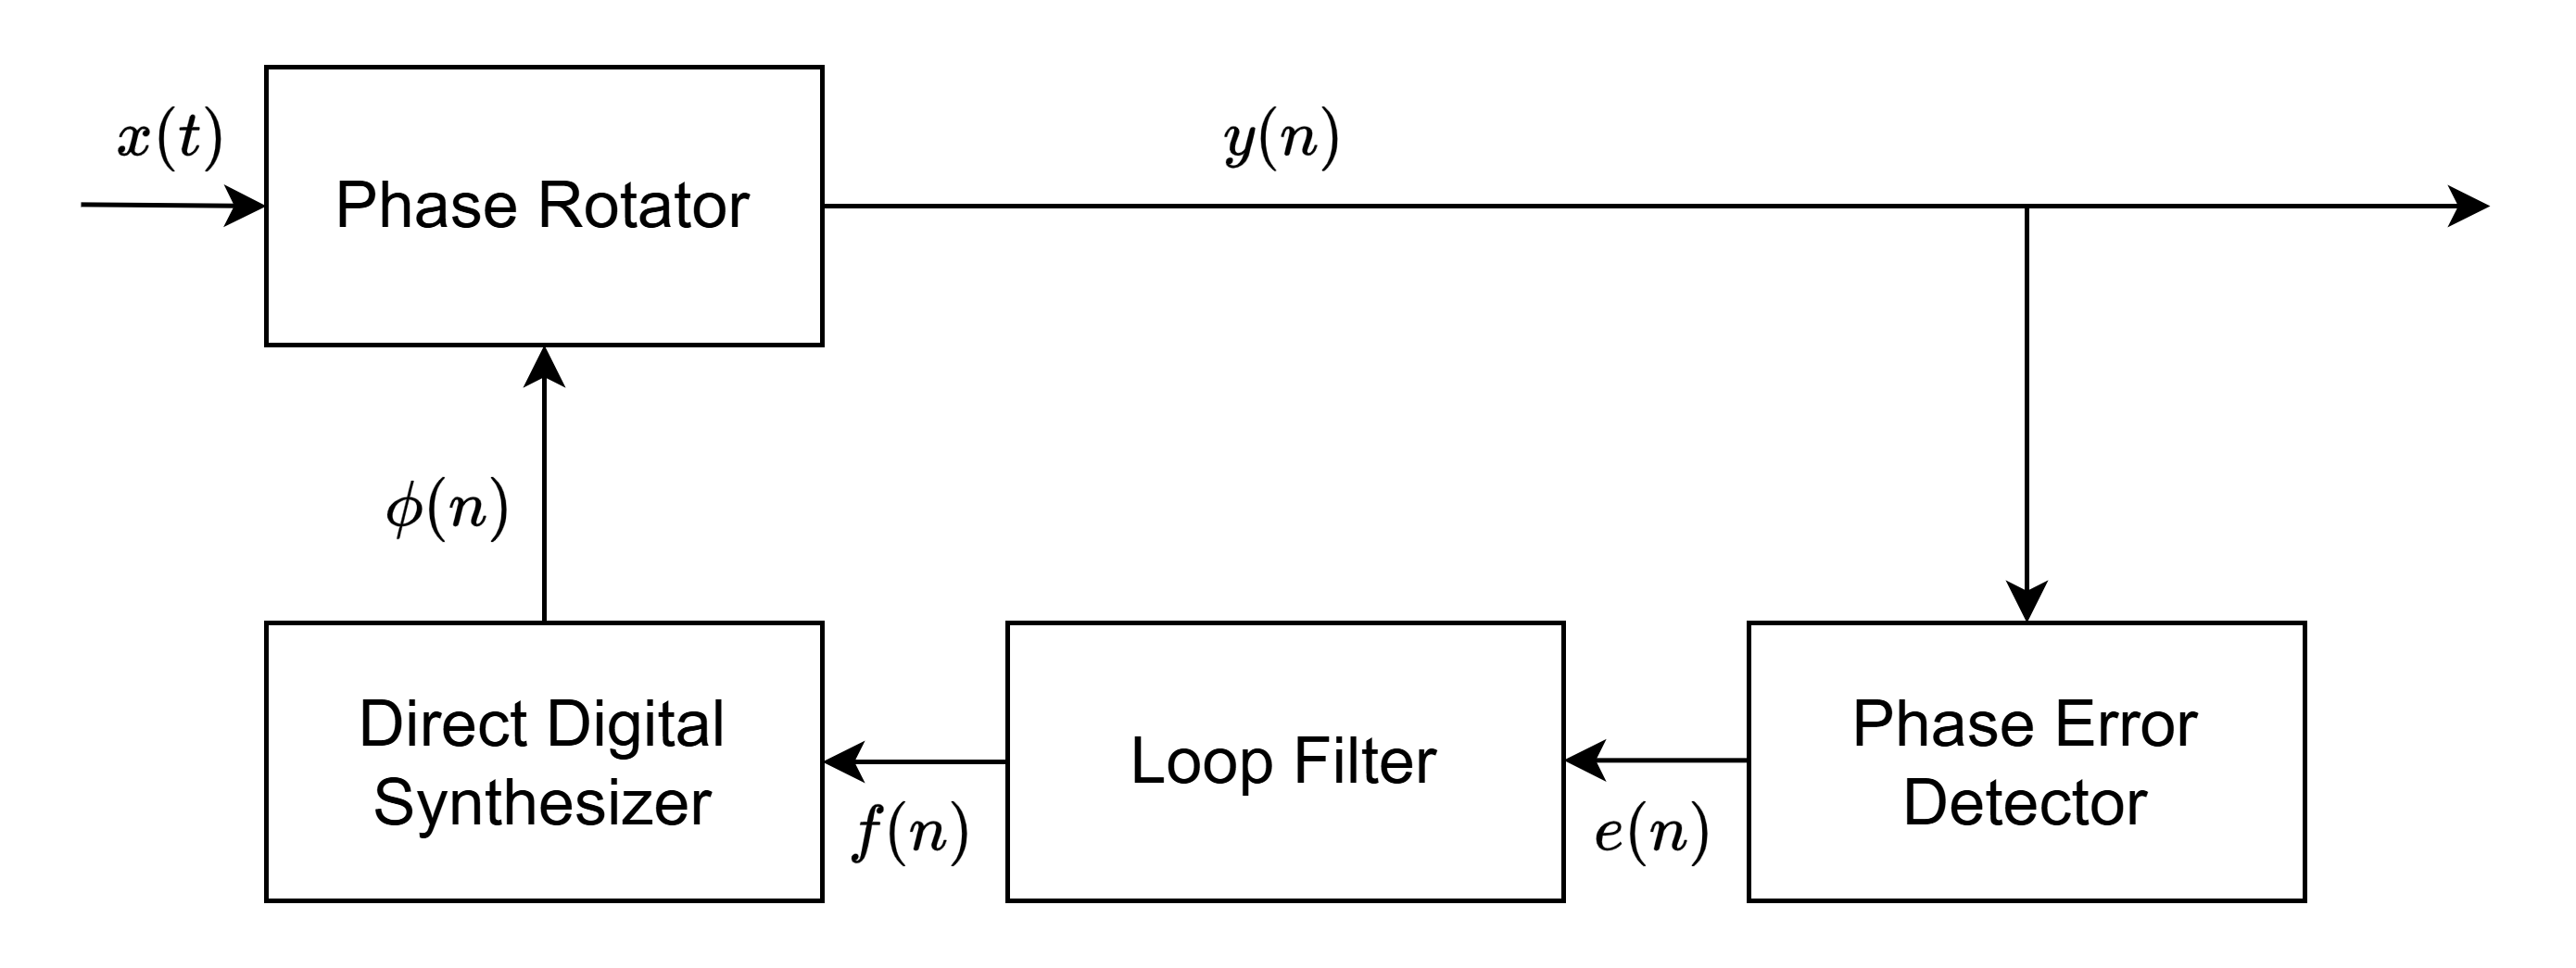
\includegraphics[width=0.5\textwidth]{carrier_synchronization.png}}}
	\caption{Fine Frequency Synchronization}
	\label{fig::carrier_synchronization}
\end{figure}

The carrier synchronization architecture is very similar to the the timing synchronization architecture. It uses a phase error detector (PED) to detect phase offsets in the received data. Then, it stabilizes the error signal in the loop filter before it is fed into a direct digital synthesizer (DDS). The DDS generates the correction signal which is applied in the phase rotator.

\subsubsection{Phase Error Detector}

The phase error detector is specific to the modulation scheme. The TDM we receive uses QPSK modulation. Therefore, we should use the compute the error signal ($e(k)$) as follows:

\begin{equation}
	e(k) = \text{sign}(\text{Re}(y(k))) \times \text{Im}(y(k)) - \text{sign}(\text{Im}(y(k))) \times \text{Re}(y(k))
\end{equation}

\noindent The error signal should be zero when, $\text{Re}(y(k)) = \pm\text{Im}(y(k))$. The algorithm should specifically try to force the received data to the nearest QPSK constellation point.

\subsubsection{Loop Filter}

The loop filter is responsible for stabilizing the error signal. It uses the same proportional-plus integrator (PI) filter that was presented in Equation \ref{eq::loop_filter} with updated values for $G_1$ and $G_2$. The updated constants are specifically defined in terms of the damping factor ($\zeta$), the loop bandwidth $B_{\text{Loop}}$, and the modulation order ($M$).

\begin{align}
	G_1 = \frac{4\zeta\theta/\Delta}{M} && G_2 = \frac{(4/M)\theta^2/\Delta}{M}
\end{align}

\noindent where $\theta$ and $\Delta$ are defined as follows:

\begin{align}
	\theta = \frac{B_{\text{Loop}}}{M(\zeta + 0.25/\zeta)} && \Delta = 1 + 2\zeta\theta + \theta^2
\end{align}

The selection of $\zeta$ affects the responsive and stability of the PLL:

\begin{equation}
\zeta = \begin{cases}
< 1, & \text{Underdamped}\\
= 1, & \text{Critically Damped}\\
> 1, & \text{Overdamped}
\end{cases}
\end{equation}

\noindent $B_\text{Loop}$ is then chosen to achieve a maximum frequency pull-in range, $\Delta_{f,\text{pull}}$, and a maximum frequency lock delay, $t_{\Delta,\text{Max}}$, which are defined in \cite{collins_2018_softwaredefined} as follows:

\begin{equation}
	\label{eq::max_freq_correct}
	\Delta_{f,\text{pull}} \sim 2\pi\sqrt{2}\zeta{B_\text{Loop}}\end{equation}

\begin{equation}
	t_{\Delta,\text{Max}} \sim \frac{32\zeta^2}{B_\text{Loop}}\end{equation}

\subsubsection{Direct Digital Synthesizer}

The direct digital synthesizer creates a tone using the phase output by the loop filter. It specifically performs phase accumulation to determine the instantaneous phase of the correction signal. The z-transform of the the DDS is specifically given by:

\begin{equation}
	D(z) = G_3\frac{z^{-1}}{1 - z^{-1}}
\end{equation}

\noindent where $G_3 = -1$ to remove the phase offset from the received signal. Note that our accumulator also includes an additional cycle of delay to simplify the implementation.

\subsubsection{Phase Rotator}

The phase rotator creates a tone from the phase output by the DDS using a lookup table (LUT). The received signal is then multiplied with the tone to remove the phase offset.

\subsection{Frame Synchronization}

XM radio divides its transmitted data into frames. These frames include two different preambles: the MFP (master frame preamble) and the FSP (fast synchronization preamble). The FSP marks the start of the data portion and corrects for ambiguities, while the MFP is used to align the signal from each satellite \cite{a2008_us8260192b2}. Both preambles and their relative timing are illustrated in Figure \ref{fig::tdm_frame_format}.

\begin{figure}[H]
	\centerline{\fbox{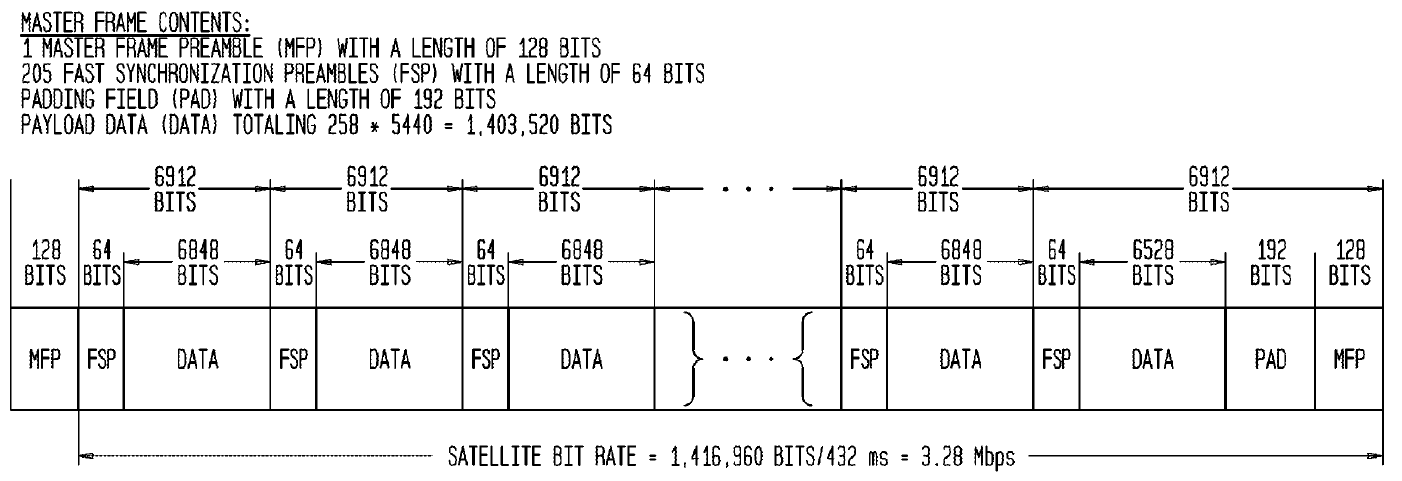
\includegraphics[width=0.8\textwidth]{tdm_frame_format.png}}}
	\caption{TDM Frame Format \cite{a2008_us8260192b2}}
	\label{fig::tdm_frame_format}
\end{figure}

\noindent We can detect both of these preambles by cross-correlating our received data with each preamble. The cross-correlation is specifically given by:

\begin{equation}
	C_{xy}(k) = \sum_m{x^*(m)y_n(m+k)}
\end{equation}

\noindent The peak of the cross-correlation output should correspond to the delay of the preamble. If the cross-correlation function is like MATLAB's \text{xcorr} function and outputs the correlation for positive and negative values of $m$, then the delay ($\hat{p}$) should be given by

\begin{equation}
	\hat{p} =  \underset{k}{\text{argmax}}\ C_{xy}(k) - L_r
\end{equation}

\noindent where $L_r$ is the length of the longest input sequence. We can also use the \texttt{filter} command to more efficiently compute the cross-correlation for short input sequences. The \texttt{filter} command performs convolution, which is given by the following formula:

\begin{equation}
	z(k) = \sum_{m}{y_n(m)h(k - m)}
\end{equation}

\noindent Therefore, to use it for cross-correlation, we need to let the filter $h(k) = x^*(-k)$.

If we threshold our 
\begin{figure}[H]
	\centerline{\fbox{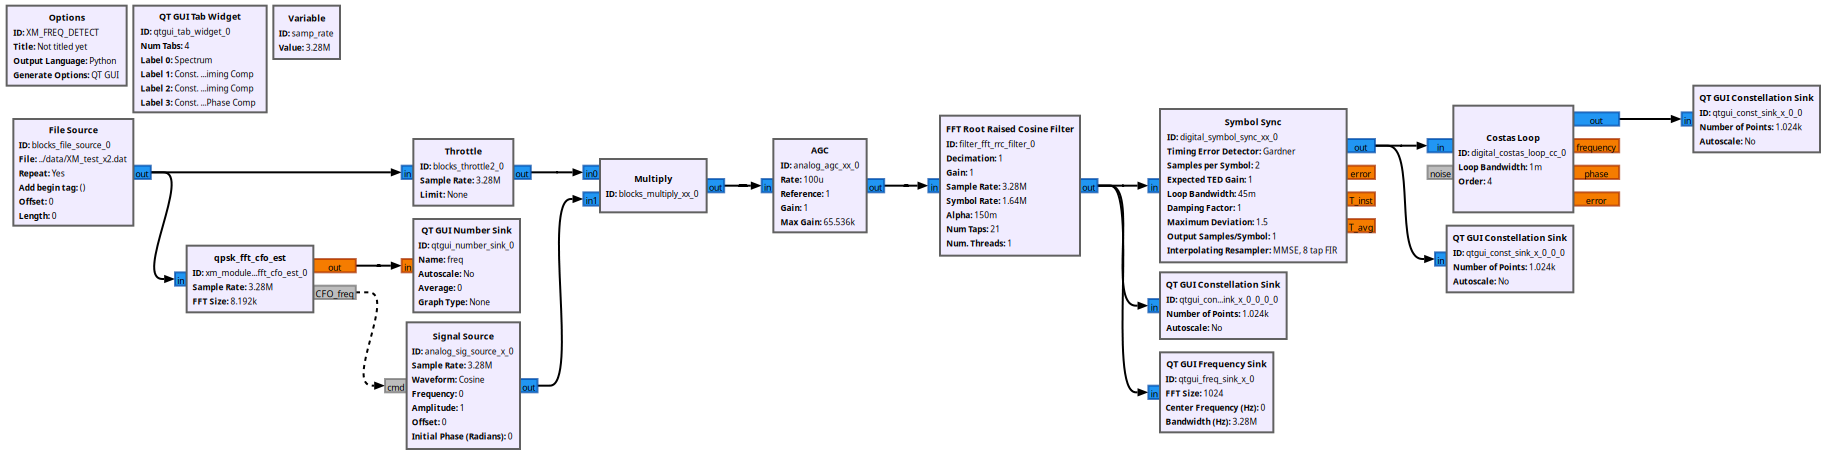
\includegraphics[width=0.8\textwidth]{timing_carrier_sync.png}}}
	\caption{GNU Radio Flowchart That Implements Timing and Carrier Synchronization}
	\label{fig::timing_carrier_sync}
\end{figure}

The XM radio signal is transmitted through a square-root raised cosine filter, which limit the signal bandwidth [ADD A CITATION HERE]. Because of this, the receiver needs a matching square root raised cosine filter. The root-raised cosine filter is a type II Nyquist filter, which results in zero intersymbol interference when the received signal is sampled at the midpoint of each symbol period. When the PlutoSDR samples the received signal, this condition is not strictly enforced. This results in significant spreading in our constellation as illustrated in Figure \ref{fig::constellation_no_timing_comp}.

\begin{figure}[H]
	\centerline{\fbox{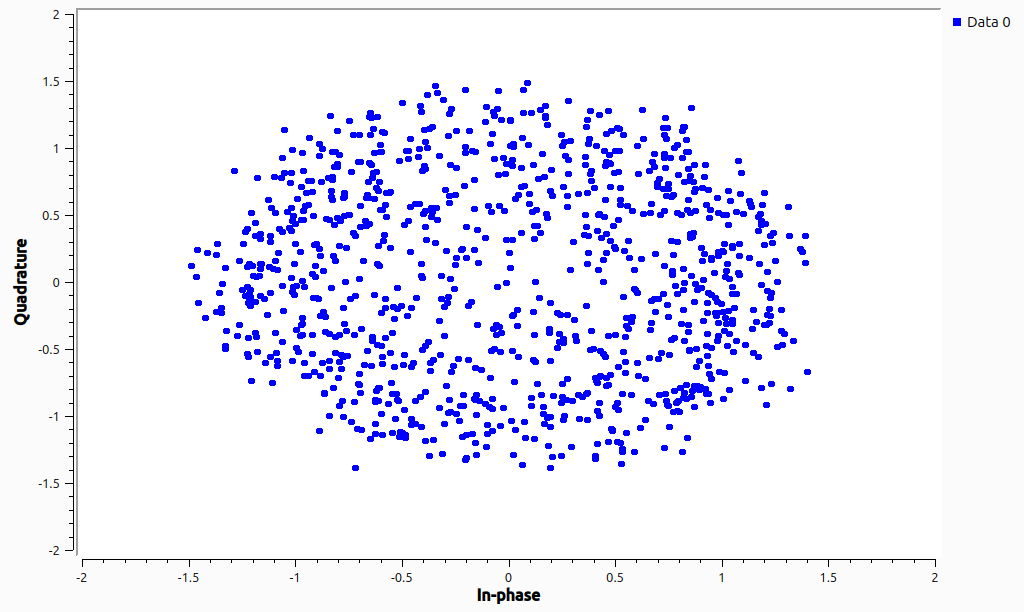
\includegraphics[width=0.5\textwidth]{constellation_no_timing_comp.png}}}
	\caption{Received Constellation Before Timing Synchronization}
	\label{fig::constellation_no_timing_comp}
\end{figure}

We can correct for this timing offset using a timing synchronization block. For this purpose, we use a GNU radio symbol sync block. This symbol sync block can be subdivided into 4 blocks: interpolator, timing error detector, loop filter, and controller. The interpolator applies a fractional delay. The timing error detector measures the timing offset. The loop filter stabilizes the process. And the controller manages the interpolation process. For our work, we specifically choose a Gardner Timing Error detector because it is robust to frequency errors. Our constellation after timing compensation is shown in Figure \ref{fig::constellation_after_timing_comp}.

\begin{figure}[H]
	\centerline{\fbox{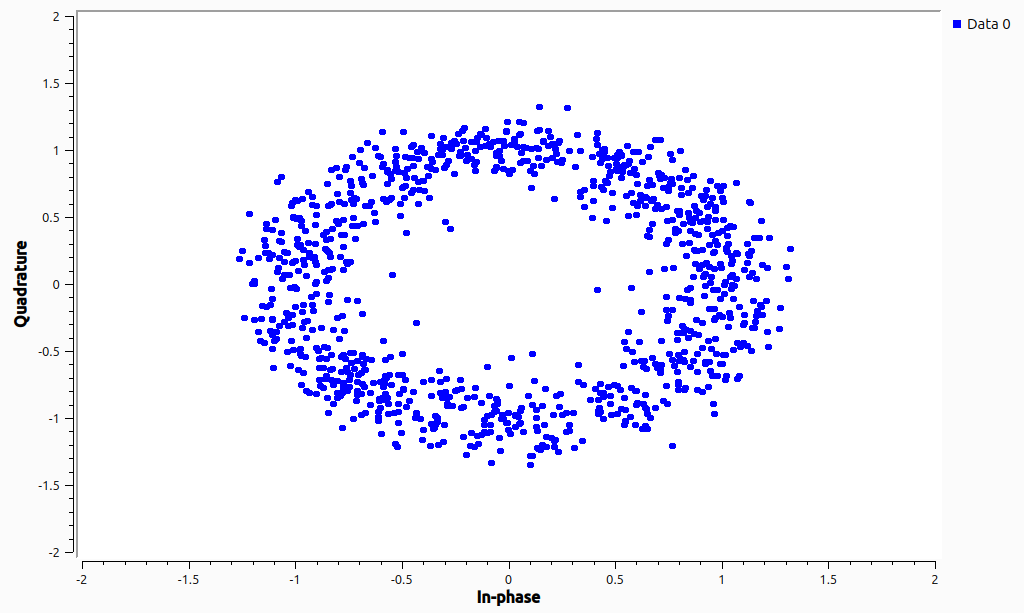
\includegraphics[width=0.5\textwidth]{constellation_after_timing_comp.png}}}
	\caption{Received Constellation After Timing Synchronization}
	\label{fig::constellation_after_timing_comp}
\end{figure}

After timing compensation, we see that the amplitude of the constellation has stabilized. However, the resulting constellation is a ring. This occurs because after phase and frequency errors. The phase error leads to a static tilt of the constellation and the frequency offset causes our constellation to rotate. To correctly demodulate the signal, we must also remove the frequency offset in the signal. We do this in 2 stages: coarse frequency compensation and fine frequency compensation. We implement the coarse frequency compensation algorithm using a custom GNU radio python block. This block raises our received data to the fourth power to remove the QPSK modulation. Then, it takes an FFT of the resulting signal. The peak index of the FFT provides us with an estimate of the coarse frequency error. When solving for the error we also must divide the frequency error by 4 to account for raising the received data to the 4th power prior to the FFT. The FFT output and the corresponding frequency error for one frame of data is shown in Figure \ref{fig::cfo_frequency_estimate}. Examining the Figure, we observe a frequency error of roughly 15 kHz [CHECK SIGN].

\begin{figure}[H]
	\centerline{\fbox{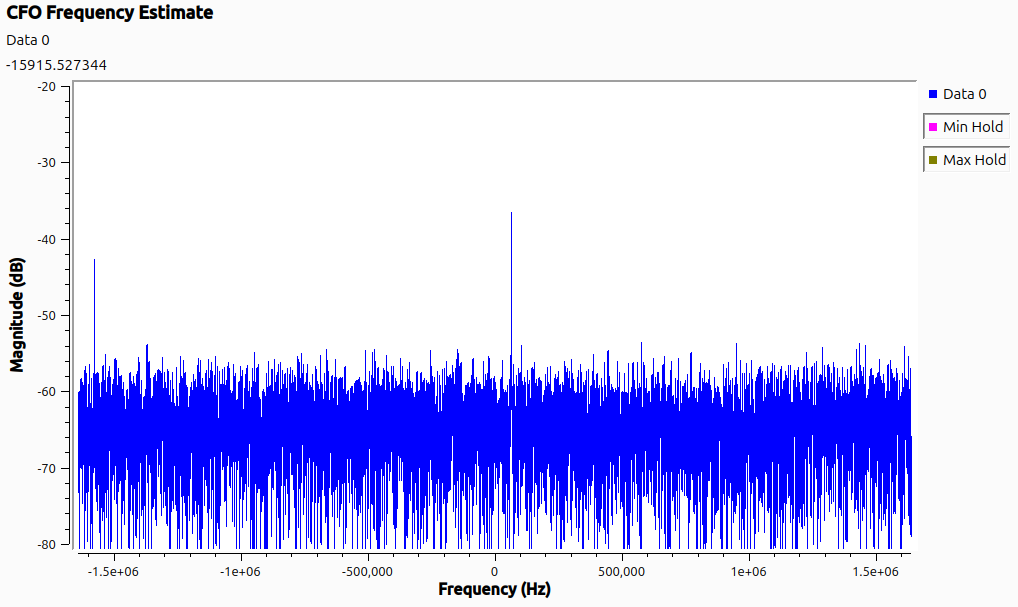
\includegraphics[width=0.5\textwidth]{cfo_frequency_estimate.png}}}
	\caption{Coarse Frequency FFT Output}
	\label{fig::cfo_frequency_estimate}
\end{figure}

The coarse frequency compensation is limited by the FFT size and the rate at which the frequency drifts. We add an additional fine frequency compensation block to resolve the rest of the error. We use the GNU radio Costas Loop block for this analysis. The GNU radio Costas Loop closely resembles the timing synchronization block. It includes a phase error detector, a loop filter, a direct digital synthesizer and a phase rotator.
The phase rotator adjusts the phase of the received signal by multiplying it with a phasor. The phase error detector then detects the phase error, which is fed into a loop filter for stabilization. Finally the Direct Digital Synthesizer creates a coherent phasor which removes residual phase and frequency offsets. The constellation after fine frequency compensation is shown in Figure \ref{fig::constellation_after_fine_carrier_comp}.

\begin{figure}[H]
	\centerline{\fbox{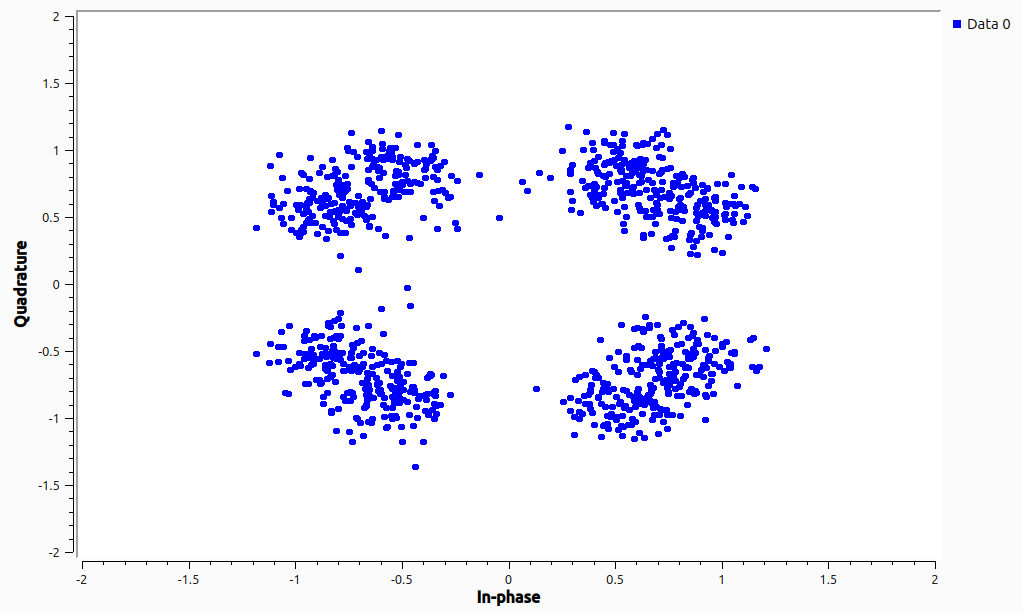
\includegraphics[width=0.5\textwidth]{constellation_after_fine_carrier_comp.png}}}
	\caption{Received Constellation After Fine Carrier Synchronization}
	\label{fig::constellation_after_fine_carrier_comp}
\end{figure}

XM radio divides its transmitted data into frames. These frames are marked by two different preambles: the MFP (master frame preamble) and the FSP (fast synchronization preamble). The FSP marks the start of the data portion and corrects for ambiguities, while the MFP is used to align the signal from each satellite \cite{a2008_us8260192b2}. Both preambles and their relative timing are illustrated in Figure \ref{fig::tdm_frame_format}.

The patents we referenced did not provide the MFP or FSP. As a result, we identified them ourselves using the auto-correlation of our signal. We considered the FSP first because it occurred more frequently in our collected data. To compute the FSP, we correlated an FSP duration of samples with a copy delayed by the FSP separation. By sweeping the starting index until we maximized the auto-correlation, we were able to effectively identify the start of our FSP. Our approach is illustrated in Figure \ref{fig::finding_fsp} and the best auto-correlation is shown in Figure \ref{fig::fsp_correlation}.

\begin{figure}[H]
	\centerline{\fbox{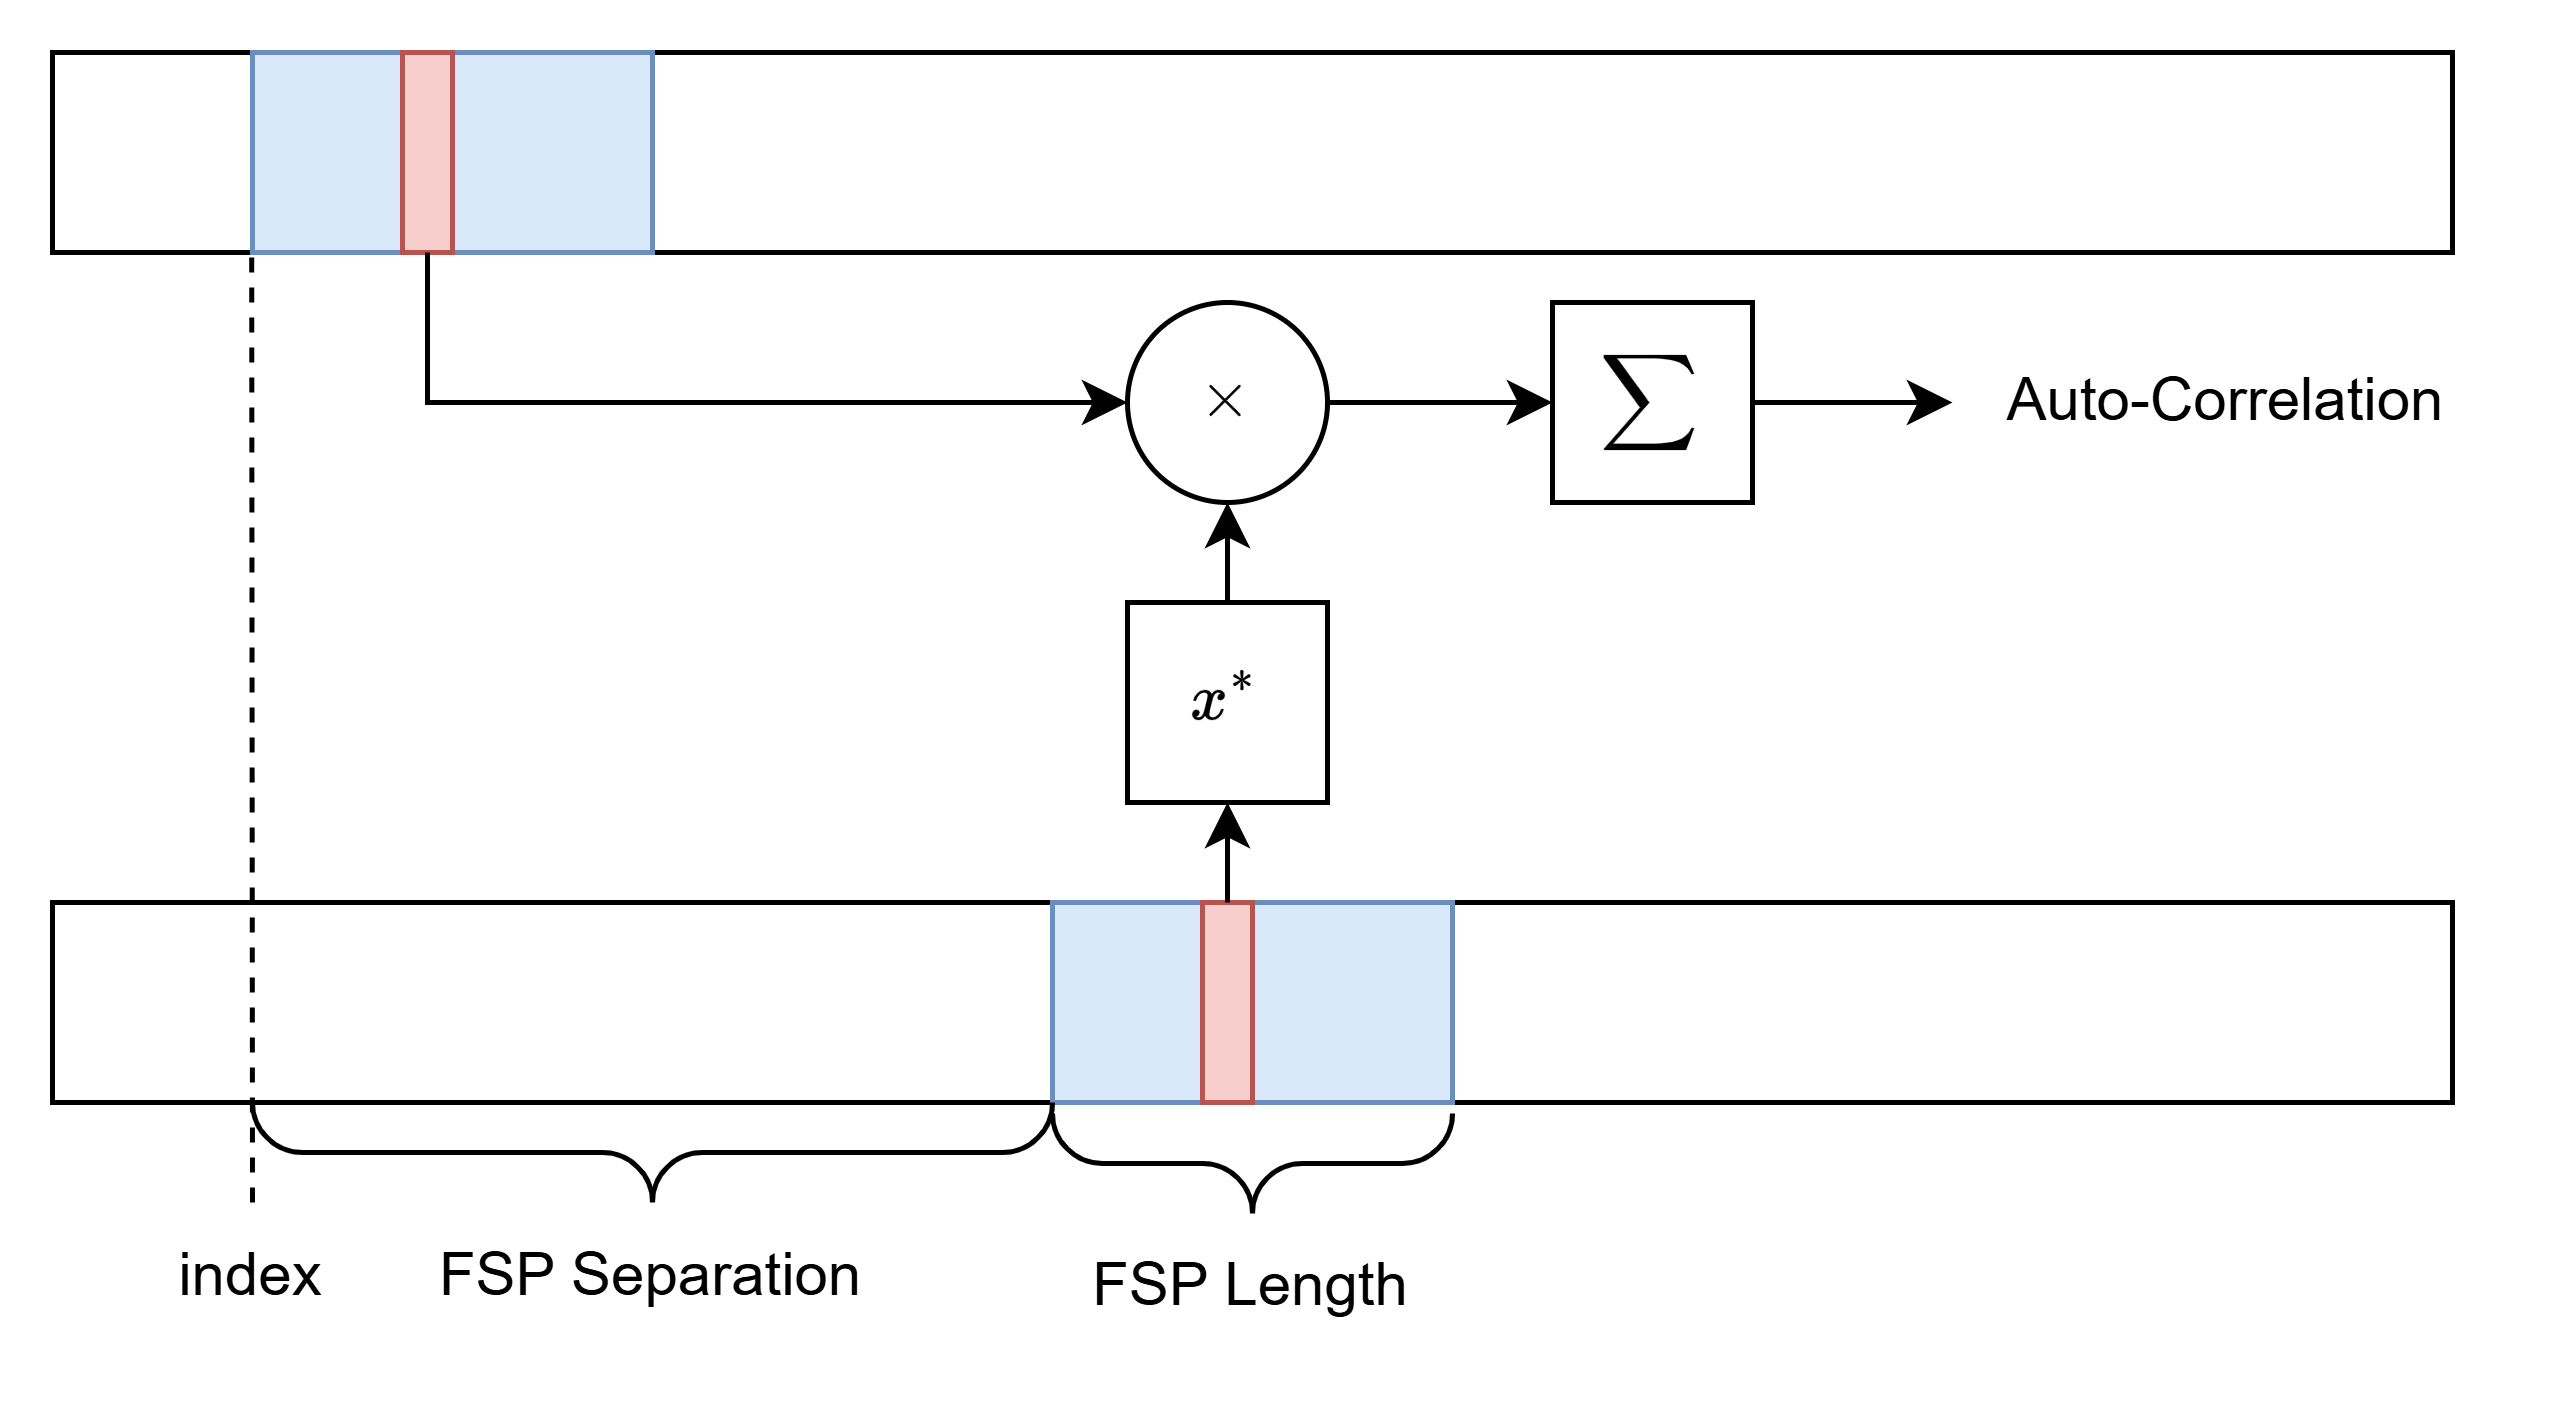
\includegraphics[width=0.5\textwidth]{finding_fsp.png}}}
	\caption{Algorithm for Indentifying FSP}
	\label{fig::finding_fsp}
\end{figure}

\begin{figure}[H]
	\centerline{\fbox{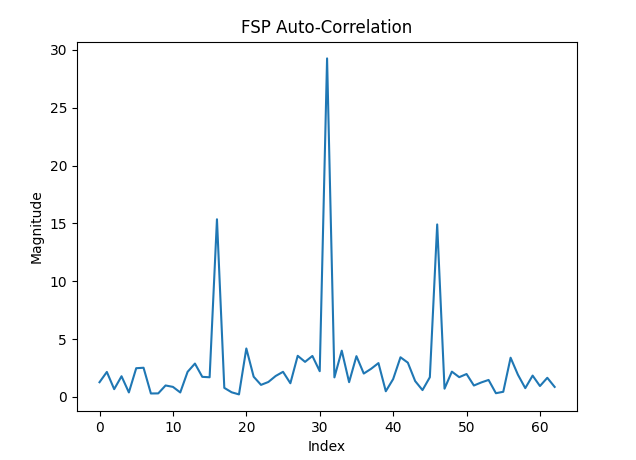
\includegraphics[width=0.5\textwidth]{fsp_correlation.png}}}
	\caption{Auto-Correlation of Optimum FSP Selection}
	\label{fig::fsp_correlation}
\end{figure}

We can also examine some of the properties of the FSP by looking at its constellation. In Figure \ref{fig::fsp_constellation}, we show the constellation of the FSP symbols and data symbols.

\begin{figure}[H]
	\centerline{\fbox{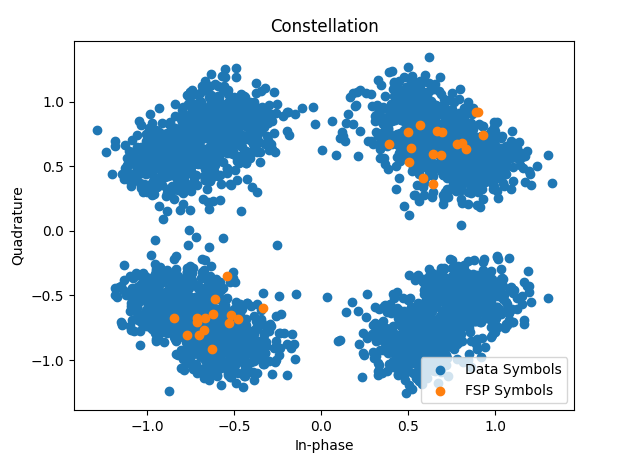
\includegraphics[width=0.5\textwidth]{fsp_constellation.png}}}
	\caption{Constellation of FSP Symbols vs Data Symbols}
	\label{fig::fsp_constellation}
\end{figure}

Examining the figure, we see that the FSP uses bi-phase modulation (phase-shifted BPSK) instead of QPSK modulation like the proceeding signals. To 
improve our correlation performance going forward, we demodulate each of the FSP constellation points. Note that our results are ambiguous by $180^{\circ}$, so we assume a leading 1 in the FSPs. Errors reported by the Reed Solomon decoder (when implemented) can be used to resolve this ambiguity. If we receive high error counts, we know to rotate the phase of our FSP by $180^{\circ}$.

We can perform a similar procedure to identify the MFP. However, to avoid false alarms from our FSP, we take advantage of the MFP located illustrated in Figure \ref{fig::tdm_frame_format}. We specifically know that the MFP will always be located right before the FSP. Therefore, we consider only MFP positions right before the FSP as illustrated in Figure \ref{fig::finding_mfp}.

\begin{figure}[H]
	\centerline{\fbox{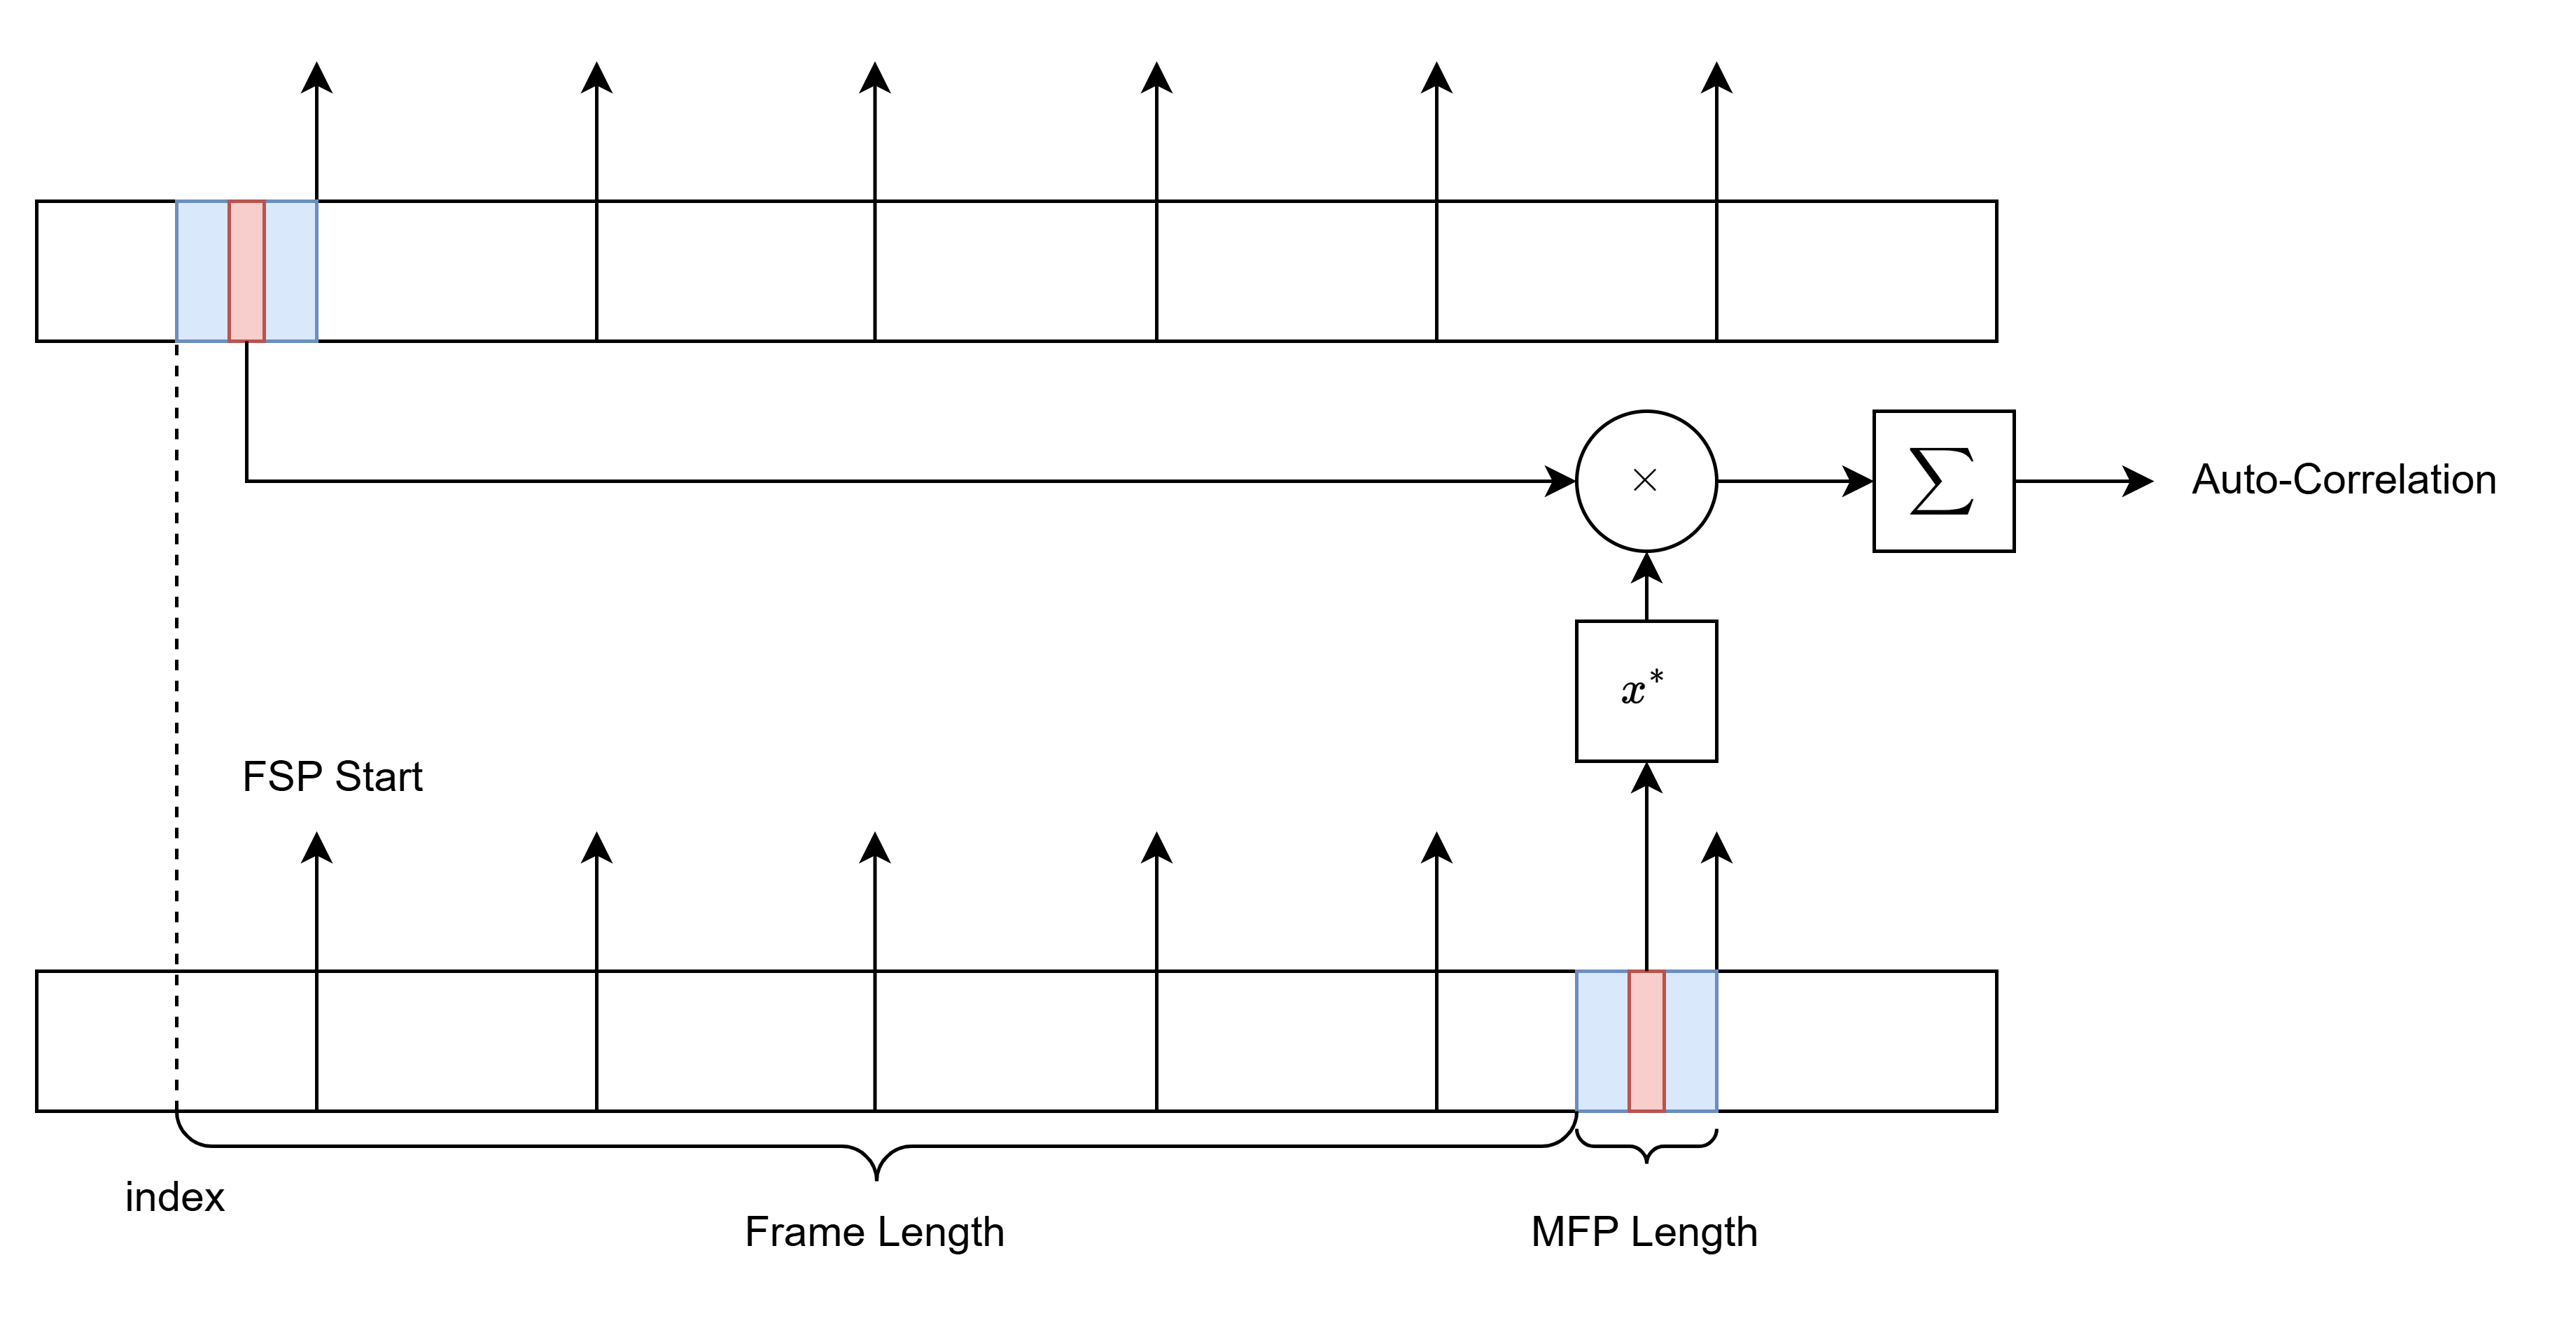
\includegraphics[width=0.5\textwidth]{finding_mfp.png}}}
	\caption{Algorithm for Indentifying MFP}
	\label{fig::finding_mfp}
\end{figure}

The base case auto-correlation provides the location of the MFP. For our data, the best case auto-correlation is shown in Figure \ref{fig::mfp_correlation} and the resulting constellation is shown in Figure \ref{fig::mfp_constellation}.

\begin{figure}[H]
	\centerline{\fbox{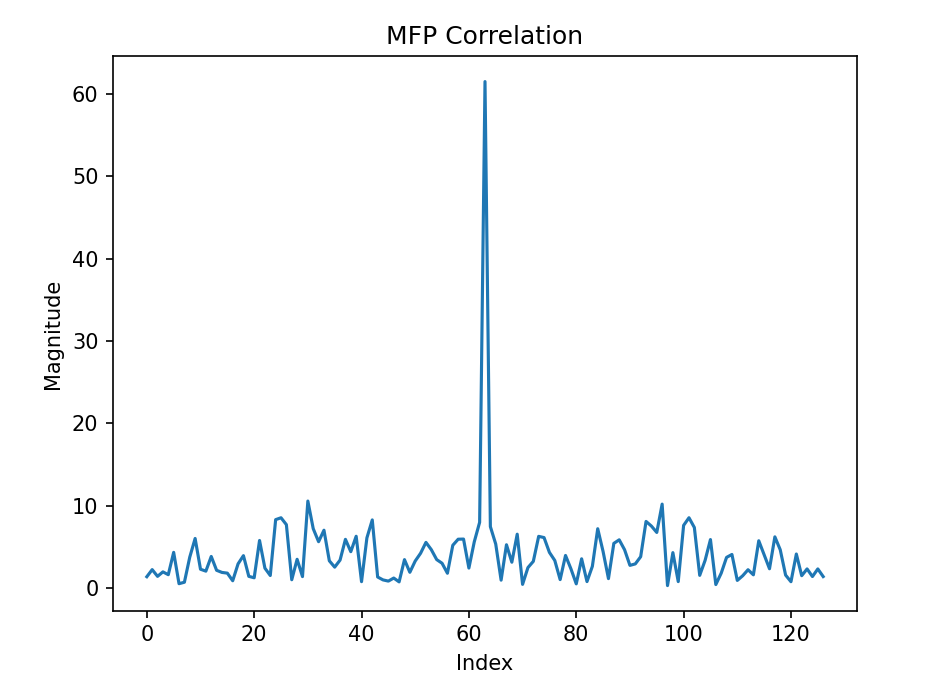
\includegraphics[width=0.5\textwidth]{mfp_correlation.png}}}
	\caption{Auto-Correlation of Optimum MFP Selection}
	\label{fig::mfp_correlation}
\end{figure}

\begin{figure}[H]
	\centerline{\fbox{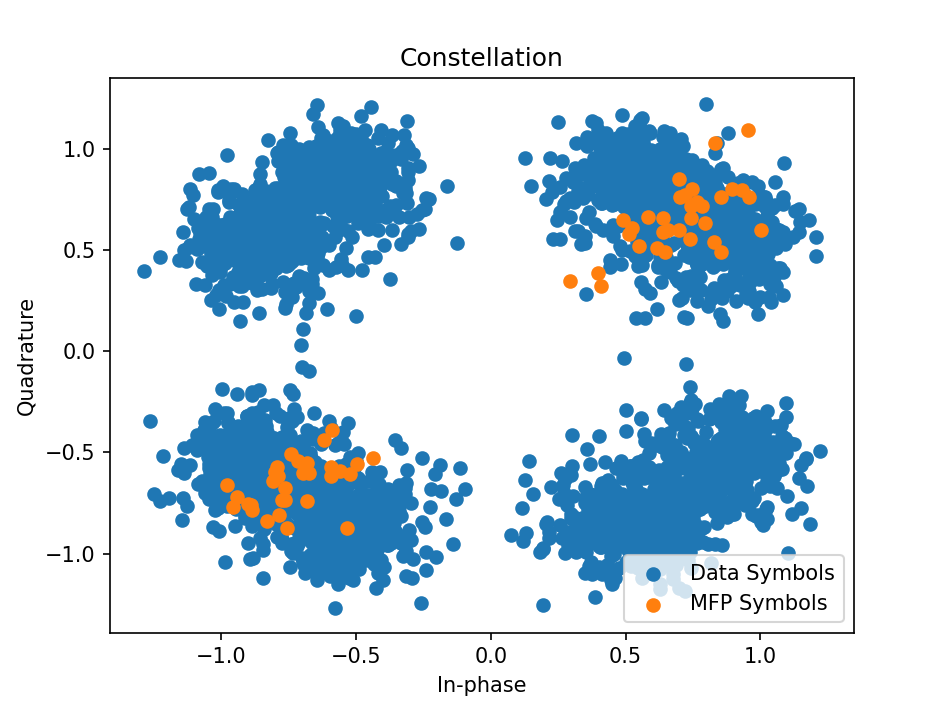
\includegraphics[width=0.5\textwidth]{mfp_constellation.png}}}
	\caption{Constellation of MFP Symbols vs Data Symbols}
	\label{fig::mfp_constellation}
\end{figure}

Examining the constellation, we see that the MFP is also bi-phase. To 
improve our correlation performance going forward, we demodulate each of the MFP constellation points. Note that our results are ambiguous by $180^{\circ}$ as described above. For now we assume a leading 1 in the MFPs.

% Add plot of FSP in constellation w/ different color

% Add picture of setup

\begin{itemize}
	\item Nyquist Filter
	\item Timing Synchronization
	\item Carrier Compensation
	\begin{itemize}
		\item Coarse
		\item Fine
	\end{itemize}
	\item Frame Synchronization
\end{itemize}

\nocite{5586866}
\nocite{a2008_us8260192b2}
\nocite{marko_2012_us8667344b2}
\nocite{collins_2018_softwaredefined}
\nocite{chaudhari_2022_timing}
\nocite{650240}
\bibliographystyle{IEEEtran}
\bibliography{sources}{}
%\bibliographystyle{ieeetr}
\end{document}